\documentclass{article}

\usepackage{graphicx}
\usepackage{tikz}
\usepackage{tikzsymbols}
\usetikzlibrary{calc,patterns,shapes.geometric}
\pagestyle{empty}
\usepackage[margin=0pt]{geometry}
\geometry{papersize={14in,12in}}

\def\centerarc[#1](#2)(#3:#4:#5){\draw[#1] ($(#2)+({#5*cos(#3)},{#5*sin(#3)})$) arc (#3:#4:#5);}

\begin{document}
	\begin{figure}
		\centering
		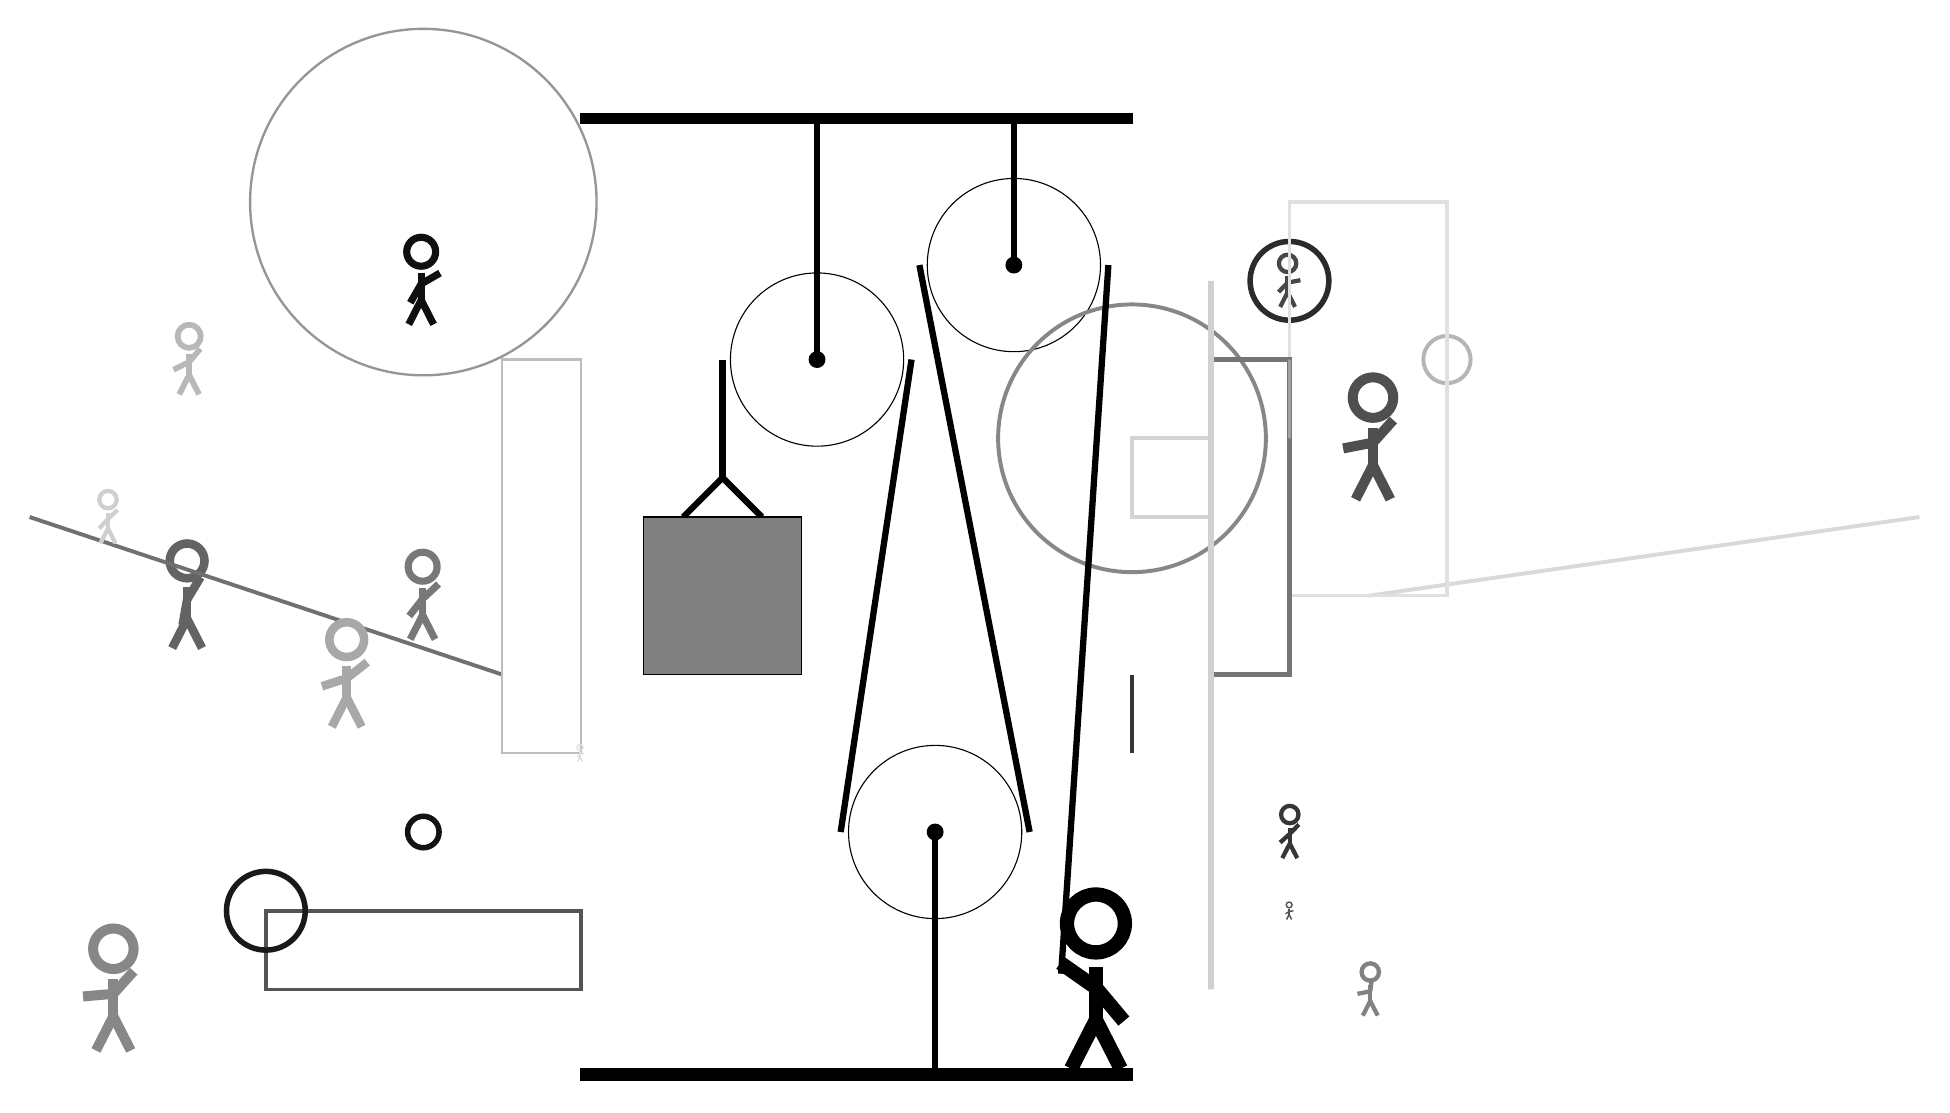
\begin{tikzpicture}
			%%%%% START %%%%%
			
			\draw[fill=black] (-2, 9) rectangle (5, 9.125);
			
			\draw (1, 6) circle (1.1);
			\draw[fill=black] (1, 6) circle (0.1);
			\draw[line width=0.8mm]  (1, 9) -- (1, 6);
			
			\draw[fill=white](2.5, 0) circle (1.1);
			\draw[fill=black] (2.5, 0) circle (0.1);
			\draw[line width=0.8mm]  (2.5, -3) -- (2.5, 0);
			
			\draw[fill=white](3.5, 7.2) circle (1.1);
			\draw[fill=black] (3.5, 7.2) circle (0.1);
			\draw[line width=0.8mm] (3.5, 9) -- (3.5, 7.2);
			
			\draw[line width=0.5mm, color=black!15](8, 3) -- (15, 4);
			
			\draw [line width=0.3mm, color=black!41](-4, 8) circle (2.2);
			\node[line width=0.7mm, color=black!68] at (7, -1) {\Strichmaxerl[1][34][7]};
			\node[line width=0.5mm, color=black!28] at (-7, 6) {\Strichmaxerl[4][26][50]};
			
			\draw [line width=0.7mm, color=black!83](7, 7) circle (0.5);
			
			\node[line width=0.2mm, color=black!47] at (-8, -2) {\Strichmaxerl[7][5][48]};
			\node[line width=0.6mm, color=black!72] at (7, 7) {\Strichmaxerl[3][46][11]};
			\node[line width=0.5mm, color=black!79] at (7, 0) {\Strichmaxerl[3][42][46]};
			\node[line width=0.7mm, color=black!61] at (-7, 3) {\Strichmaxerl[6][80][59]};
			
			\draw[line width=0.5mm, color=black!56](-3, 2) -- (-9, 4);
			
			\node[line width=0.6mm, color=black!49] at (8, -2) {\Strichmaxerl[3][11][83]};
			\draw [line width=0.5mm, color=black!29](9, 6) circle (0.3);
			\draw[line width=0.5mm, color=black!67] (-2, -1) rectangle (-6, -2);
			
			\draw[line width=0.3mm, color=black!26] (-3, 6) rectangle (-2, 1);
			\node[line width=0.3mm, color=black!19] at (-8, 4) {\Strichmaxerl[3][48][43]};
			\draw[line width=0.5mm, color=black!17] (5, 5) rectangle (6, 4);
			
			\draw[line width=0.4mm, color=black!12] (7, 3) rectangle (9, 8);
			
			\node[line width=0.6mm, color=black!34] at (-5, 2) {\Strichmaxerl[6][18][38]};
			\node[line width=0.2mm, color=black!94] at (-4, 7) {\Strichmaxerl[5][60][30]};
			\node[line width=0.5mm, color=black!13] at (-2, 1) {\Strichmaxerl[1][49][8]};
			\draw [line width=0.5mm, color=black!47](5, 5) circle (1.7);
			
			\node[line width=0.2mm, color=black!53] at (-4, 3) {\Strichmaxerl[5][52][43]};
			\draw[line width=0.7mm, color=black!54] (7, 6) rectangle (6, 2);
			\draw [line width=0.7mm, color=black!93](-4, 0) circle (0.2);
			\draw [line width=0.7mm, color=black!94](10, 3) circle (0.0);
			
			\draw[line width=0.7mm, color=black!18] (6, -2) rectangle (6, 7);
			\draw[line width=0.5mm, color=black!79](5, 1) -- (5, 2);
			\draw [line width=0.7mm, color=black!90](-6, -1) circle (0.5);
			
			\node[line width=0.2mm, color=black!69] at (8, 5) {\Strichmaxerl[7][11][48]};
			\draw[line width=0.4mm, color=black!37] (7, 6) rectangle (7, 5);
			
			\draw[line width=0.8mm] (-0.7, 4.0) -- (-0.2, 4.5) -- (0.3, 4.0);
			\draw[fill=black!50] (-1.2, 4.0) rectangle (0.8, 2.0);
			
			\draw[line width=0.8mm] (-0.2, 6) -- (-0.2, 4.5);
			\centerarc[line width=0.8mm](1, 6)(0:180:1.2000000000000002);
			\draw[line width=0.8mm](2.2, 6) -- (1.3, 0);
			\centerarc[line width=0.8mm](2.5, 0)(180:360:1.2000000000000002);
			\draw[line width=0.8mm](3.7, 0) -- (2.3, 7.2);
			\centerarc[line width=0.8mm](3.5, 7.2)(0:180:1.2000000000000002);
			\draw[line width=0.8mm](4.7, 7.2) -- (4.1, -1.8);
			
			\node at (4.5, -1.9) {\Strichmaxerl[10][-35][-50]};
			
			\draw[fill=black] (-2, -3) rectangle (5, -3.15);
			
			%%%%% END %%%%%
		\end{tikzpicture}
	\end{figure}	
\end{document}